\documentclass[11pt,a4paper]{article}
\usepackage[T1]{fontenc}
\usepackage[utf8]{inputenc}
\usepackage{lmodern}
\usepackage[a4paper,left=2.2cm,right=2.2cm,top=2cm,bottom=2cm]{geometry}
\usepackage{graphicx,xcolor,booktabs,tabularx,array}
\usepackage{microtype,fancyhdr,titlesec,enumitem,float,caption,listings,xurl}
\usepackage[unicode,colorlinks=true,linkcolor=teal,urlcolor=teal]{hyperref}
\definecolor{ink}{HTML}{183B50}
\definecolor{teal}{HTML}{14675F}
\definecolor{paper}{HTML}{F1F5F7}
\definecolor{line}{HTML}{B8C9D1}
\hypersetup{pdftitle={Laporan Praktikum Web Service Lab 09 - Microservices},
 pdfauthor={Bambang Herlambang},pdfsubject={Praktikum individu - NRP 5803024019}}
\graphicspath{{images/}}
\pagestyle{fancy}
\fancyhf{}
\fancyfoot[C]{\small\color{ink}\thepage}
\renewcommand{\headrulewidth}{0pt}
\renewcommand{\footrulewidth}{0pt}
\titleformat{\section}{\large\bfseries\color{ink}}{\thesection.}{0.5em}{}
\titleformat{\subsection}{\normalsize\bfseries\color{ink}}{\thesubsection}{0.5em}{}
\titlespacing*{\section}{0pt}{8pt}{7pt}
\titlespacing*{\subsection}{0pt}{8pt}{4pt}
\setlength{\parindent}{0pt}
\setlength{\parskip}{5pt}
\setlength{\intextsep}{6pt}
\setlength{\textfloatsep}{8pt}
\setlength{\emergencystretch}{2em}
\renewcommand{\arraystretch}{1.17}
\renewcommand{\figurename}{Gambar}
\renewcommand{\tablename}{Tabel}
\captionsetup{font=small,labelfont=bf,labelsep=period,skip=5pt,justification=raggedright,singlelinecheck=false}
\setlist[itemize]{leftmargin=1.3em,itemsep=2pt,topsep=3pt}
\setlist[enumerate]{leftmargin=1.6em,itemsep=3pt,topsep=4pt}
\newcolumntype{L}[1]{>{\raggedright\arraybackslash}p{#1}}
\newcolumntype{Y}{>{\raggedright\arraybackslash}X}
\newcommand{\code}[1]{\texttt{\detokenize{#1}}}
\newcommand{\repo}{\href{https://github.com/academicbambang/prakwebservice-lab09-microservices}{prakwebservice-lab09-microservices}}
\lstset{basicstyle=\small\ttfamily,backgroundcolor=\color{paper},
 frame=single,rulecolor=\color{line},breaklines=true,columns=fullflexible,
 keepspaces=true,showstringspaces=false,aboveskip=6pt,belowskip=6pt,
 xleftmargin=7pt,xrightmargin=7pt,framexleftmargin=5pt,framexrightmargin=5pt}
% Generated from the actual local test log and smoke-test JSON.
\newcommand{\LocalTestCount}{67}
\newcommand{\LocalPassCount}{67}
\newcommand{\LocalFailCount}{0}
\newcommand{\DemoTimestamp}{2026-10-28T09:32:19.961Z}
\newcommand{\DemoLocalTime}{28 Oktober 2026 pukul 16:32:19}
\newcommand{\SmokeProductCount}{3}
\newcommand{\SmokeOrderStatus}{201}
\newcommand{\SmokeStockBefore}{40}
\newcommand{\SmokeStockAfter}{38}
\newcommand{\SmokeTotal}{170.000}

\begin{document}
\hypersetup{pageanchor=false}
\begin{titlepage}
\newgeometry{left=2.5cm,right=2.5cm,top=2.5cm,bottom=2.5cm}
\thispagestyle{empty}
{\fontfamily{ptm}\selectfont\fontsize{12}{16}\selectfont
\centering
{\bfseries LAPORAN PRAKTIKUM WEB SERVICE\par}
\vspace{0.8cm}
{\bfseries SESI 09: MEMECAH APLIKASI\par}
{\bfseries MENJADI MICROSERVICES\par}
\vspace{0.9cm}

\includegraphics[width=7.8cm,height=7.8cm,keepaspectratio]{logo-ukwms.png}\par
\vspace{0.8cm}
{\bfseries DISUSUN OLEH\par}
\vspace{0.3cm}
Bambang Herlambang\par
NRP 5803024019\par
\vspace{0.25cm}
Praktikum Individu\par
28 Oktober 2026\par
\vfill
{\bfseries
PROGRAM STUDI INFORMATIKA\par
FAKULTAS TEKNIK\par
UNIVERSITAS KATOLIK WIDYA MANDALA\par
SURABAYA\par
2026\par}
}
\end{titlepage}
\restoregeometry
\setcounter{page}{1}
\hypersetup{pageanchor=true}

\section{Tujuan dan ruang lingkup}
Praktikum ini memisahkan pengelolaan produk dan stok dari pengelolaan pesanan.
Catalog Service menjadi satu-satunya pemilik data produk, sedangkan Order
Service menyimpan riwayat pesanan dan meminta reservasi stok melalui HTTP.
API Gateway menjadi pintu masuk bersama untuk kedua service.

Pengerjaan dilakukan secara individu pada repository khusus Lab 09,
\repo. Gateway dipakai ulang dari
\href{https://github.com/academicbambang/prakwebservice-lab08-api-gateway}{implementasi Lab 08}.
Contoh produk memakai konteks Marketplace UMKM Kelompok D; laporan ini
mencatat implementasi praktikum individu dan pemetaan fiturnya ke rancangan proyek.

Nama folder \code{catalog-service} dipertahankan dari kode sumber dan berperan
sebagai \textit{product-service} pada materi. Data memakai ID
\code{prod-001} dan body pesanan \code{customerName/items}, menggantikan contoh
ID angka dan \code{productId/qty} tanpa mengubah prinsip pemisahan service.

\begin{figure}[H]
\centering
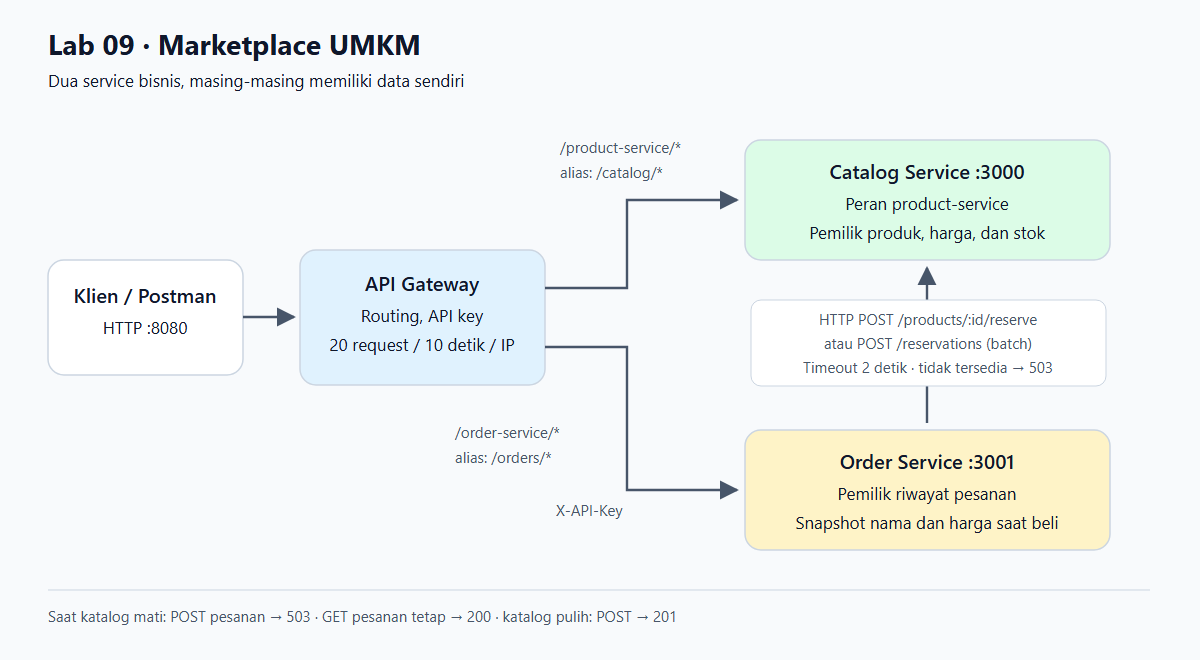
\includegraphics[width=\linewidth]{arsitektur.png}
\caption{Arsitektur microservices: data produk dan pesanan dimiliki service
yang berbeda. Reservasi stok dilakukan melalui HTTP dengan timeout dua detik.}
\end{figure}

\textbf{Kriteria utama.} Pesanan sukses mengurangi stok; kegagalan katalog
menghasilkan POST pesanan \code{503}; GET pesanan tetap \code{200}; dan
pembuatan pesanan pulih menjadi \code{201} setelah katalog hidup kembali.

\clearpage
\section{Monolit, batas service, dan kepemilikan data}
\subsection{Baseline sebelum dipisah}
Folder \code{monolith} menyediakan contoh satu proses yang menyimpan array
produk dan pesanan. Handler \code{POST /orders} membaca harga, memeriksa
stok, dan langsung mengurangi \code{product.stock}. Ketika proses ini mati,
akses produk dan pesanan berhenti bersama.

\begin{lstlisting}
npm install
npm run setup
npm run start:monolith
\end{lstlisting}

Uji \code{GET /products}, buat pesanan dua kopi, lalu baca
\code{GET /products/prod-001}: stok awal 40 menjadi 38. Hentikan monolit
sebelum menjalankan katalog pada port 3000.

\subsection{Pemetaan ke proyek Marketplace UMKM}
\begin{table}[H]
\small
\begin{tabularx}{\linewidth}{@{}L{2.6cm}Y Y@{}}
\toprule
Service & Data dan tanggung jawab & API dan komunikasi \\
\midrule
Catalog / Product &
Produk, kategori, penjual, harga, stok tersedia. Satu-satunya pemilik stok. &
Daftar/detail produk, GraphQL, reservasi satu produk dan batch. Dipanggil
Order Service saat membuat pesanan. \\
Order &
Pelanggan, jumlah barang, total, status, waktu, dan salinan nama/harga saat pembelian. &
Daftar/detail/buat pesanan. Memanggil reservasi katalog lewat HTTP; tidak
mengimpor data katalog. \\
API Gateway &
Konfigurasi route, API key, dan penghitung rate limit; tanpa data bisnis. &
Meneruskan request klien ke service setelah pemeriksaan gateway. \\
\bottomrule
\end{tabularx}
\caption{Batas service berdasarkan data dan tanggung jawab.}
\end{table}

\subsection{Alur sesudah dipisah}
\begin{enumerate}
\item Klien mengirim pesanan melalui gateway dengan API key.
\item Order Service memvalidasi body dan menggabungkan quantity produk yang berulang.
\item Order Service meminta reservasi ke katalog melalui HTTP.
\item Katalog memvalidasi seluruh stok sebelum menguranginya, lalu mengembalikan salinan produk.
\item Order Service menghitung harga dari respons katalog dan menyimpan pesanan.
\end{enumerate}

Salinan nama dan harga membuat riwayat pesanan tidak berubah ketika data
produk berikutnya berubah. Data tetap in-memory dan direset ketika proses
pemiliknya dimulai ulang.

\clearpage
\section{Kontrak API dan implementasi}
\subsection{Route melalui gateway}
Default gateway adalah \code{http://127.0.0.1:8080}; katalog pada port
3000 dan pesanan pada port 3001. Prefix gateway dihapus sebelum request
diteruskan. Alias asal \code{/catalog/*} dan \code{/orders/*} tetap tersedia.

\begin{table}[H]
\small
\begin{tabularx}{\linewidth}{@{}L{1.3cm}Y L{1.5cm}@{}}
\toprule
Method & Path pada gateway & Status normal \\
\midrule
GET & \path{/product-service/products} & 200 \\
GET & \path{/product-service/products/:id} & 200 \\
POST & \path{/product-service/products/:id/reserve} & 200 \\
POST & \path{/product-service/reservations} & 200 \\
GET & \path{/order-service/orders} & 200 \\
GET & \path{/order-service/orders/:id} & 200 \\
POST & \path{/order-service/orders} & 201 \\
\bottomrule
\end{tabularx}
\caption{Endpoint utama Lab 09. Reservasi dan route pesanan memerlukan
\code{X-API-Key} pada gateway; pembacaan katalog tidak.}
\end{table}

\subsection{Reservasi dan penanganan error}
Reservasi tunggal memakai \code{POST /products/:id/reserve} dengan body
\code{{"qty":2}}. Pesanan dengan beberapa jenis produk memakai
\code{POST /reservations}; seluruh item diperiksa sebelum mutasi sehingga
penolakan satu produk tidak memotong stok produk lain.

Order Service membatasi panggilan katalog, termasuk pembacaan body,
selama dua detik. Gangguan jaringan atau timeout menjadi \code{503}.
Produk tidak dikenal diteruskan sebagai \code{404}; stok tidak cukup
sebagai \code{409}; input tidak valid sebagai \code{400}. Respons upstream
yang rusak ditolak agar tidak menjadi sumber harga pesanan.

\subsection{Contoh body pesanan}
\begin{lstlisting}
{
  "customerName": "Bambang",
  "items": [
    { "productId": "prod-001", "quantity": 2 }
  ]
}
\end{lstlisting}
Harga kopi berasal dari katalog, yaitu Rp85.000 per unit. Dua unit
menghasilkan total Rp170.000; kolom harga atau total yang dikirim klien
tidak dipakai sebagai sumber perhitungan.

\clearpage
\section{Menjalankan, Postman, dan prosedur pengujian}
\subsection{Menyiapkan aplikasi}
Gunakan Node.js 22 atau lebih baru dari root repository:
\begin{lstlisting}
npm install
npm run setup
npm start
\end{lstlisting}
Setup membuat key lokal dalam \code{gateway/.env}. Isi hanya variabel
\code{apiKey} lokal di Postman; jangan menampilkan nilainya pada screenshot.

\subsection{Collection Postman JSON}
Import \path{docs/postman/lab09.postman_collection.json} dan environment
\path{docs/postman/lab09.postman_environment.json}. Collection berisi 14
request dalam tiga kelompok: alur normal, input negatif, lalu kegagalan
dan pemulihan. Semua request klien menuju gateway.

Alur normal membuktikan tiga produk tersedia, POST pesanan diterima,
stok turun dua, dan riwayat tersimpan. Skenario negatif menguji quantity
nol, produk tidak dikenal, stok tidak cukup, serta penolakan reservasi.
Kelompok kegagalan dijalankan manual dengan intervensi untuk mematikan dan
menghidupkan katalog di antara request.

\subsection{Otomatis dan manual}
\begin{lstlisting}
npm test
npm run test:lab09
\end{lstlisting}
Suite otomatis menggunakan assertion atas respons HTTP. Demo
\code{test:lab09} menyiapkan tiga proses pada port lokal yang tersedia,
merekam smoke test, menghentikan hanya katalog, lalu menghidupkannya kembali.
Untuk stack yang sedang berjalan, \code{npm run test:smoke} membuat
pesanan sungguhan dan mengurangi stok.

Uji kegagalan manual memakai tiga terminal:
\begin{lstlisting}
node catalog-service/server.js
node order-service/server.js
node gateway/gateway.js
\end{lstlisting}
Hentikan hanya terminal katalog, lakukan POST dan GET pesanan, lalu
hidupkan kembali katalog sebelum mengulangi POST. Launcher
\code{npm start} menutup seluruh stack jika satu child keluar, sehingga
launcher tersebut tidak dipakai untuk mematikan satu service secara manual.
Rate limit gateway tetap 20 request per 10 detik per IP.

\clearpage
\section{Hasil pengujian lokal}
\subsection{Ringkasan assertion dan smoke test}
Log \path{docs/evidence/lab09/tests.txt} mencatat
\textbf{\LocalPassCount\ test lulus dari \LocalTestCount, \LocalFailCount\ gagal}.
Skenario mencakup stok, produk berulang, batch, pesanan bersamaan, GraphQL,
API key, route gateway, timeout, dan isolasi kegagalan.

Demo direkam pada \textbf{\DemoLocalTime\ UTC+7}, dengan timestamp sumber
\texttt{\DemoTimestamp}. Tiga proses lokal terpisah menjalankan katalog,
pesanan, dan gateway.

\begin{table}[H]
\begin{tabularx}{\linewidth}{@{}Y L{4.6cm}@{}}
\toprule
Pemeriksaan & Hasil aktual \\
\midrule
Jumlah produk & \SmokeProductCount \\
POST pesanan & HTTP \SmokeOrderStatus \\
Stok kopi sebelum / sesudah & \SmokeStockBefore\ / \SmokeStockAfter \\
Total pesanan & Rp\SmokeTotal \\
Katalog berhenti: POST / GET pesanan & HTTP 503 / HTTP 200 \\
Katalog hidup kembali: POST pesanan & HTTP 201 \\
Jumlah pesanan setelah pemulihan & 2, termasuk pesanan sebelum gangguan \\
\bottomrule
\end{tabularx}
\caption{Ringkasan bukti smoke test dan kegagalan service.}
\end{table}

\subsection{Asal screenshot}
Empat screenshot pada halaman berikut merupakan tangkapan browser atas
halaman bukti otomatis \path{docs/evidence/lab09/index.html}. Halaman itu
menampilkan request dan respons HTTP aktual dari skrip Node.js melalui
gateway lokal. \textbf{Gambar tersebut bukan screenshot Postman.}
Collection Postman disediakan untuk mengulangi pengujian secara manual.

Header request yang berisi API key tidak disimpan pada JSON, log, atau
halaman bukti. Port dipilih otomatis, sehingga berbeda dari port default
aplikasi. Screenshot dan JSON harus berasal dari demo yang sama; menjalankan
ulang skrip menuntut pengambilan screenshot baru.

\clearpage
\subsection{Bukti smoke test}
Tiga produk berhasil dibaca melalui gateway. Pesanan dua kopi diterima
dengan \code{201}; stok berkurang dari 40 menjadi 38, dengan total Rp170.000.
\begin{figure}[H]
\centering
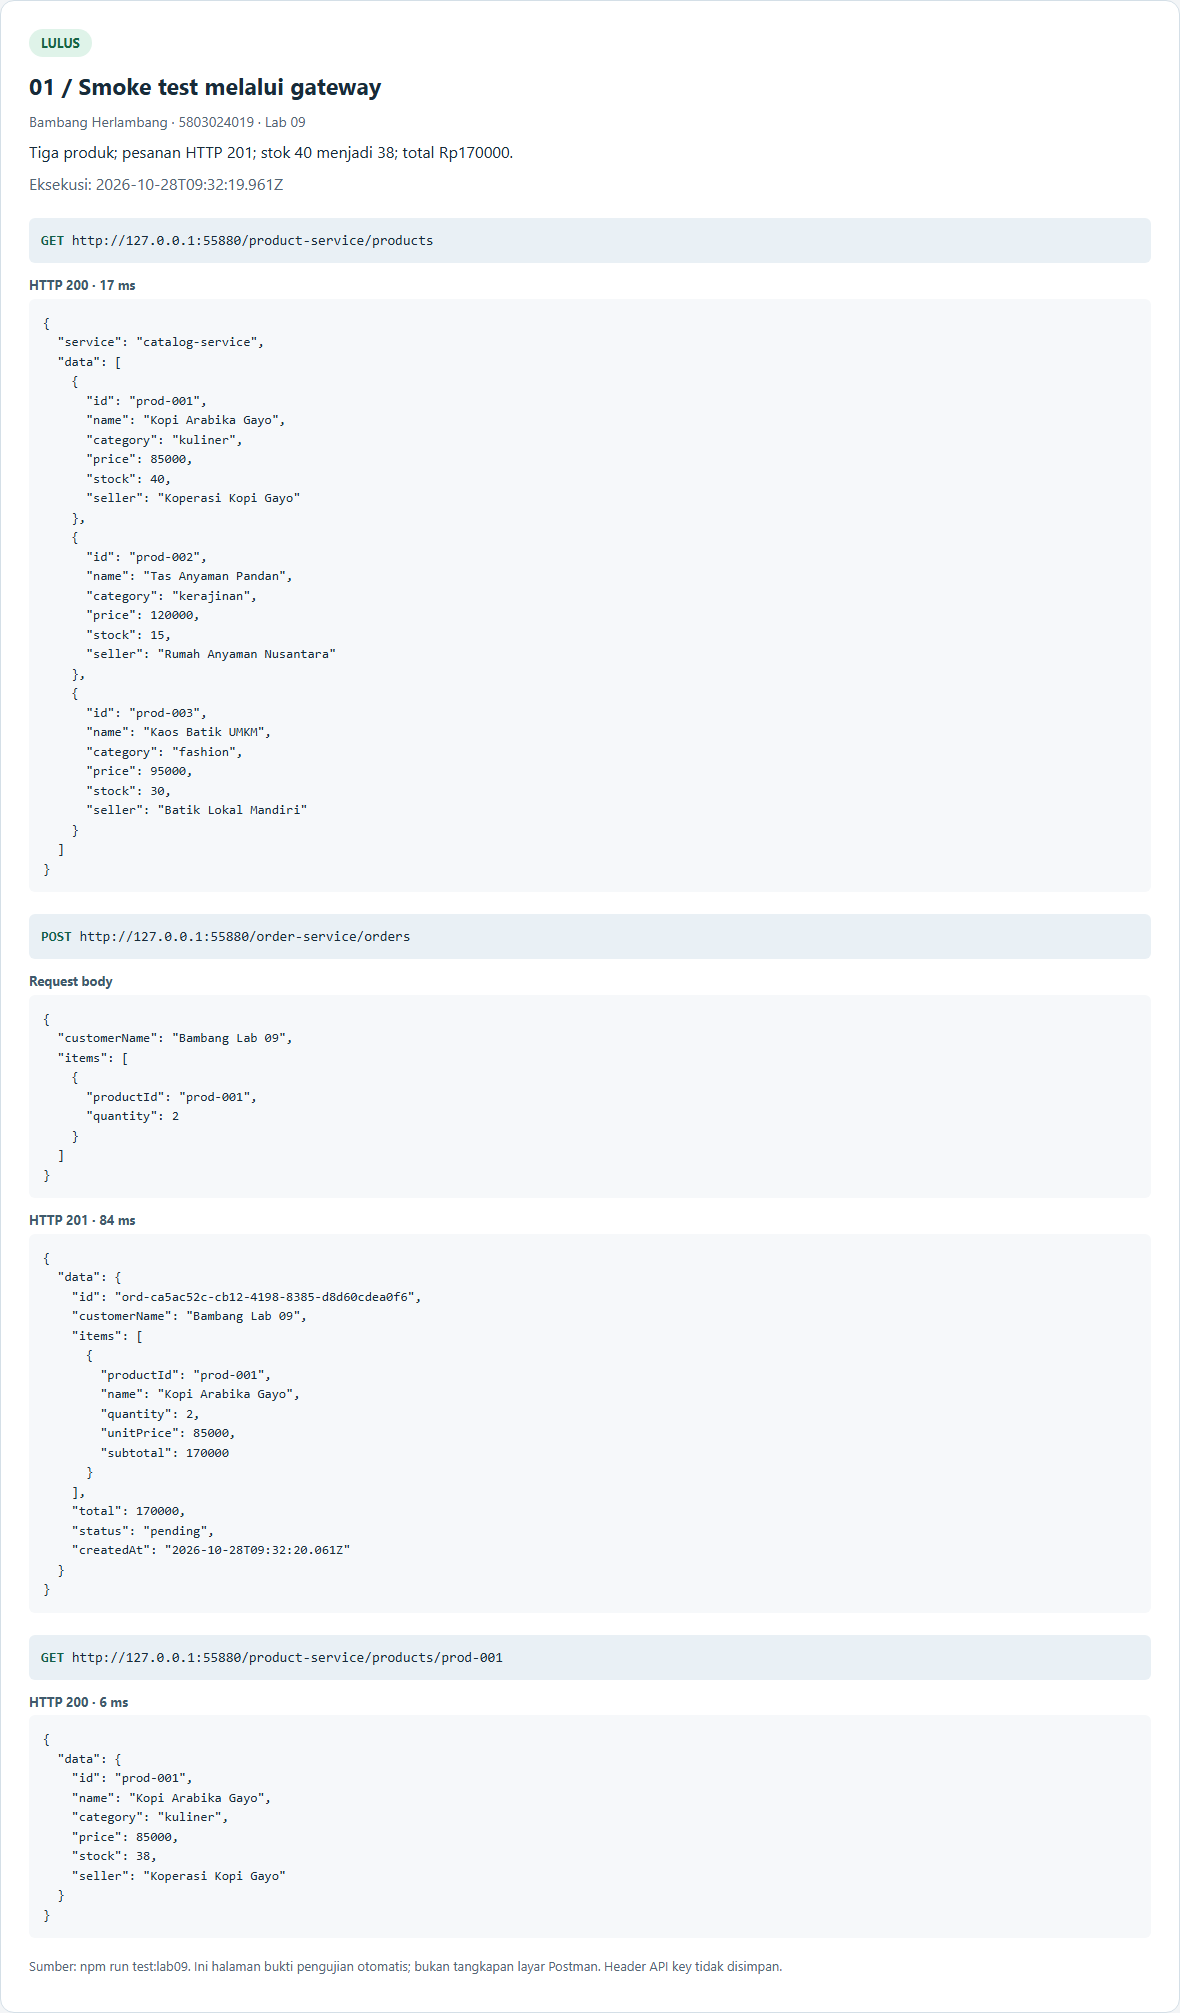
\includegraphics[width=.89\linewidth,height=.78\textheight,keepaspectratio]{smoke-test.png}
\caption{Respons HTTP aktual smoke test melalui gateway lokal.}
\end{figure}

\clearpage
\subsection{POST saat katalog berhenti}
Skrip menghentikan hanya proses katalog. Gateway dan Order Service tetap
berjalan. Pembuatan pesanan gagal dengan \code{503}, disertai pesan yang jelas.
\begin{figure}[H]
\centering
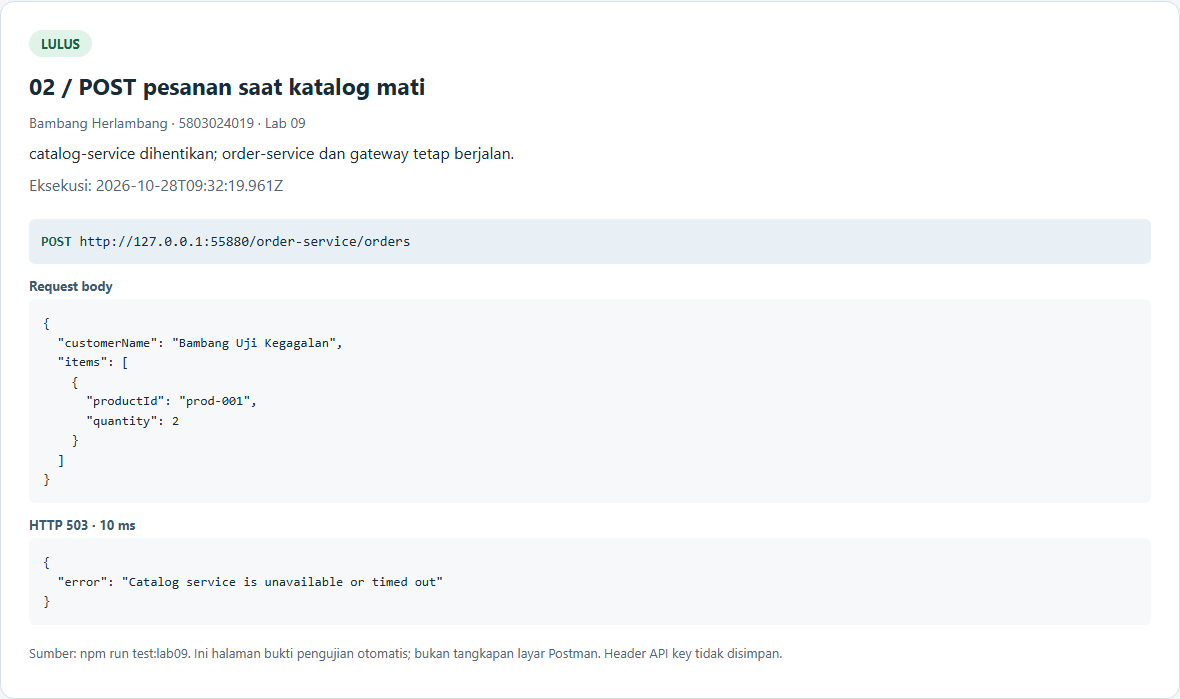
\includegraphics[width=\linewidth,height=.65\textheight,keepaspectratio]{product-down-post.png}
\caption{POST pesanan menjadi 503 saat Catalog Service tidak tersedia.}
\end{figure}
POST yang ditolak tidak menambahkan pesanan. Pemeriksaan berikutnya
membaca daftar pesanan langsung dari Order Service untuk membuktikan
bahwa kegagalan katalog tidak menghentikan seluruh sistem.

\clearpage
\subsection{GET saat katalog masih berhenti}
Order Service tetap dapat menampilkan pesanan dari smoke test tanpa
menghubungi katalog. Respons \code{200} berikut membuktikan riwayat pesanan
tetap tersedia pada proses yang sama.
\begin{figure}[H]
\centering
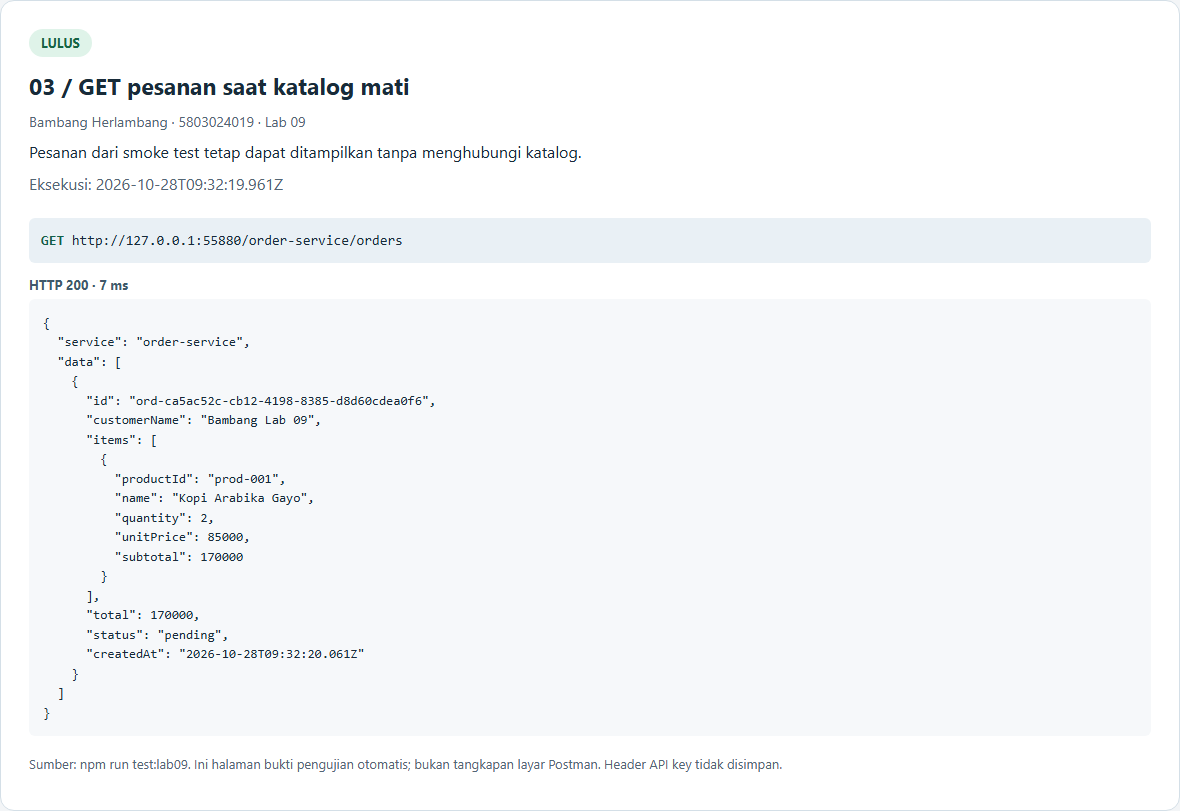
\includegraphics[width=\linewidth,height=.69\textheight,keepaspectratio]{product-down-get.png}
\caption{GET pesanan tetap 200 dan memuat pesanan sebelum gangguan.}
\end{figure}

\clearpage
\subsection{POST setelah katalog hidup kembali}
Hanya katalog yang dihidupkan kembali. Fixture katalog dimulai dari stok
40; POST pesanan baru diterima dengan \code{201} dan stok menjadi 38.
Order Service tetap menyimpan pesanan sebelum gangguan.
\begin{figure}[H]
\centering
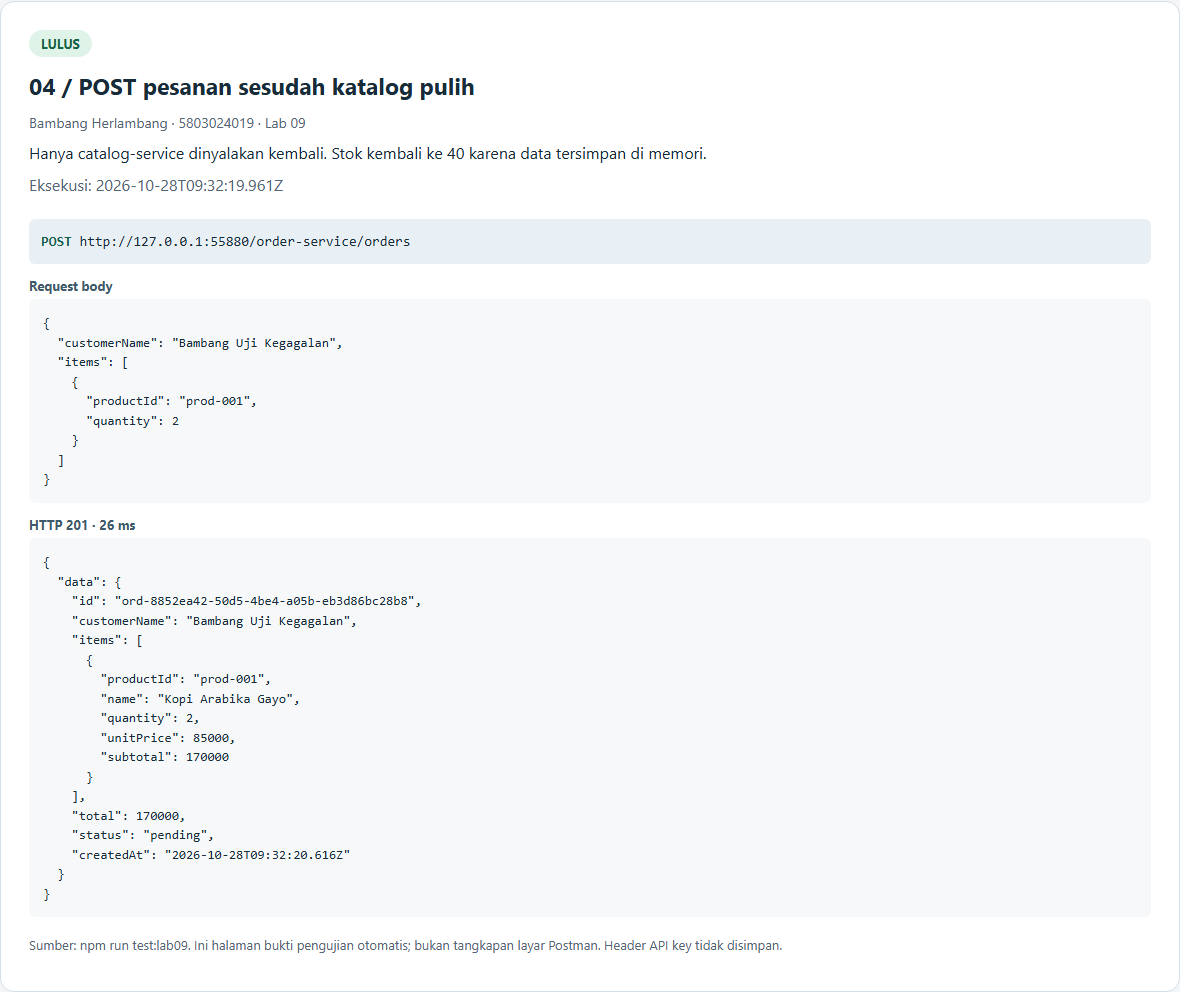
\includegraphics[width=.96\linewidth,height=.73\textheight,keepaspectratio]{product-recovered-post.png}
\caption{Pembuatan pesanan pulih menjadi 201 setelah katalog berjalan kembali.}
\end{figure}

\clearpage
\section{Frontend, dokumentasi interaktif, dan deployment}
\subsection{Frontend Ruang UMKM}
Frontend pada route \code{/} menghubungkan katalog, keranjang, pembuatan
pesanan, dan riwayat melalui gateway yang sama. Halaman menyediakan tiga
produk, perubahan quantity, total perkiraan, nama pemesan, serta input API
key untuk operasi pesanan. Harga akhir dan ketersediaan stok tetap
ditentukan service, bukan nilai yang ditampilkan klien.

\begin{figure}[H]
\centering
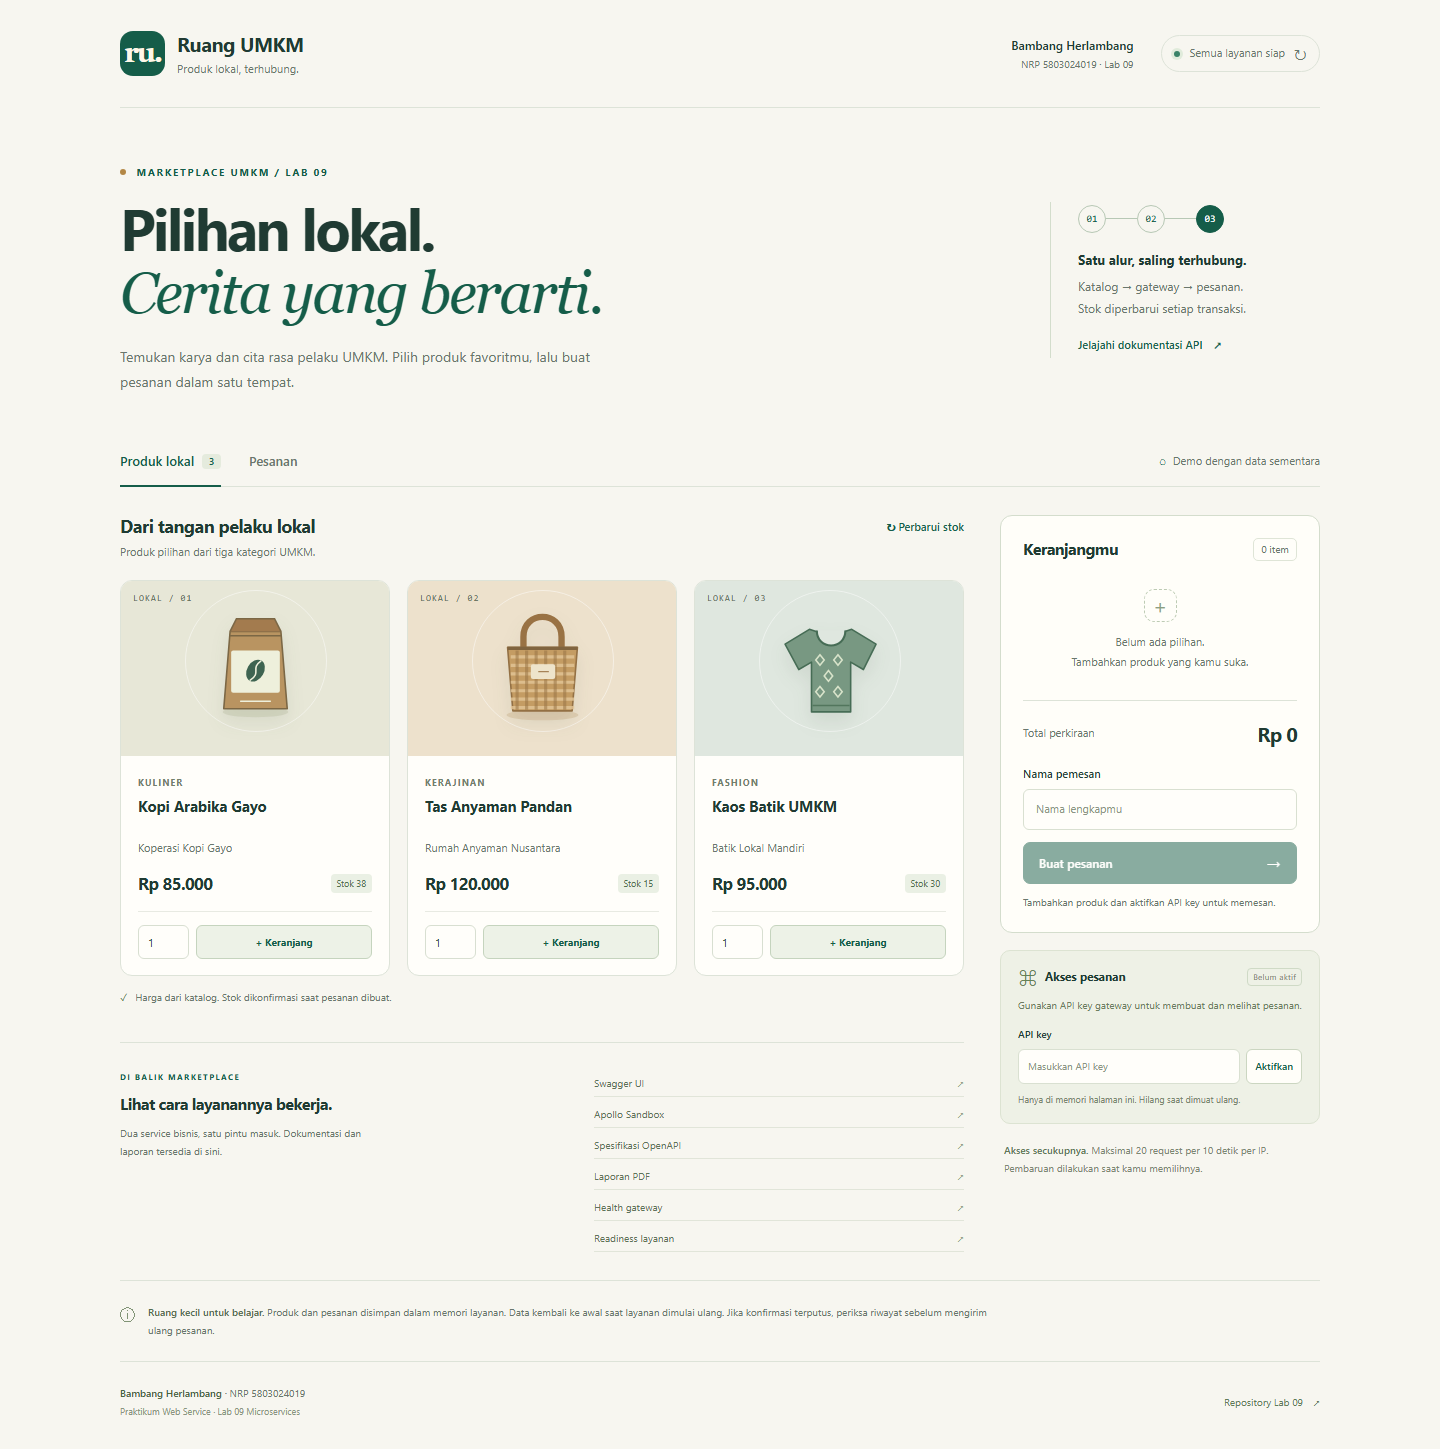
\includegraphics[width=\linewidth,height=.66\textheight,keepaspectratio]{frontend.png}
\caption{Frontend lokal Ruang UMKM: daftar produk, keranjang, dan akses
pesanan. Key belum diaktifkan pada tangkapan ini.}
\end{figure}

Tautan Swagger UI, Apollo Sandbox, OpenAPI JSON, laporan PDF, health, dan
readiness tersedia dari halaman. API key hanya disimpan dalam memori sesi
halaman; tidak ditulis ke localStorage atau sessionStorage.

\clearpage
\subsection{Checkout dan riwayat pesanan}
Pengujian browser lokal mencatat checkout dua kopi berhasil: stok yang
terbaca sebelum transaksi adalah 38 dan setelah transaksi 36. Pengujian
ini terpisah dari smoke test 40 menjadi 38 pada bagian sebelumnya.
Halaman riwayat menampilkan pesanan, rincian barang, harga, dan status.

\begin{figure}[H]
\centering
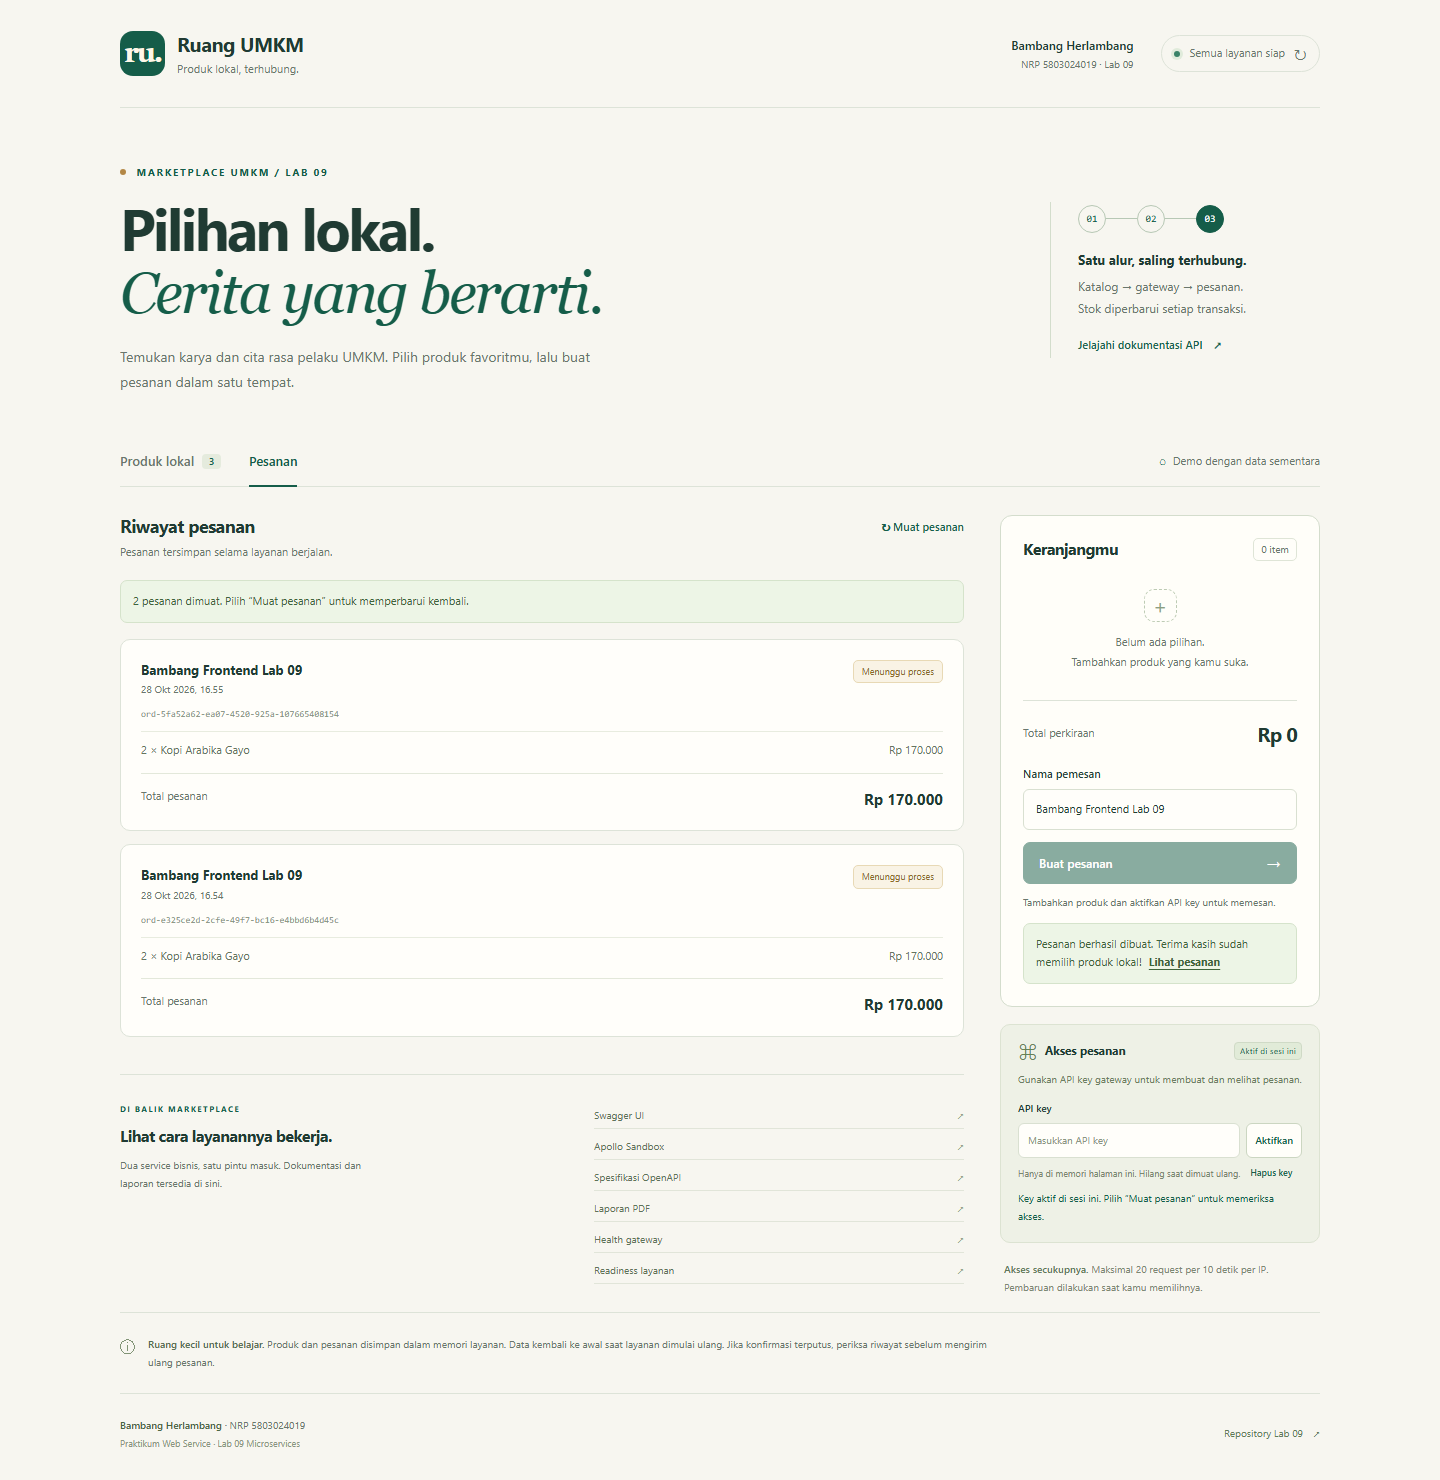
\includegraphics[width=\linewidth,height=.69\textheight,keepaspectratio]{frontend-orders.png}
\caption{Riwayat pesanan lokal setelah checkout melalui frontend. Nilai
key tidak ditampilkan; halaman menggunakan kredensial sesi sementara.}
\end{figure}

Rekaman \path{docs/evidence/ui/ui-verification.json} memuat hasil checkout,
penolakan API key salah, pengujian mobile, Swagger, dan pemuatan iframe
Apollo. Pengujian browser tersebut tidak mencatat page error.

\clearpage
\subsection{Tampilan mobile dan key tidak valid}
Pada viewport 390 piksel, verifikasi browser tidak menemukan overflow
horizontal. Produk, keranjang, form pesanan, dan navigasi disusun ulang
untuk layar sempit. Key salah ditolak dan halaman menampilkan pesan
kegagalan tanpa menyimpan nilai key dalam browser storage.

\begin{figure}[H]
\centering
\begin{minipage}[t]{.48\linewidth}
\centering
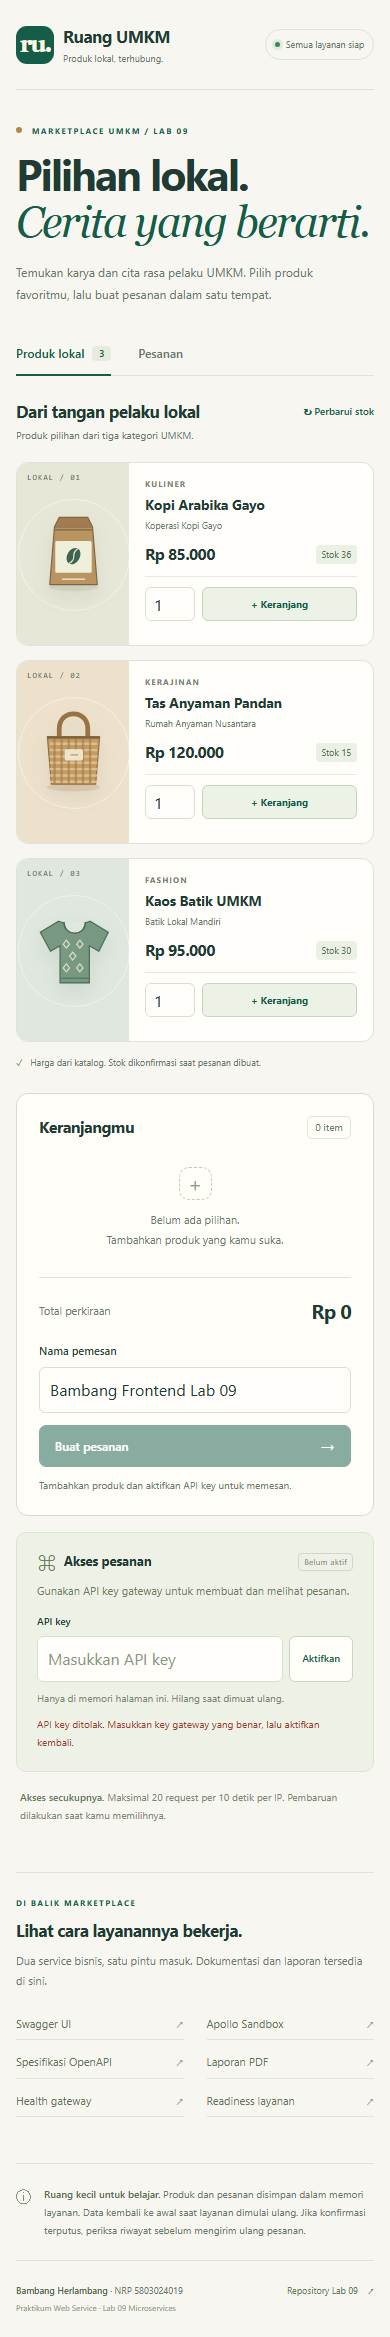
\includegraphics[width=.78\linewidth,height=.70\textheight,keepaspectratio,trim=0 1087bp 0 0,clip]{frontend-mobile.png}
\end{minipage}\hfill
\begin{minipage}[t]{.48\linewidth}
\centering
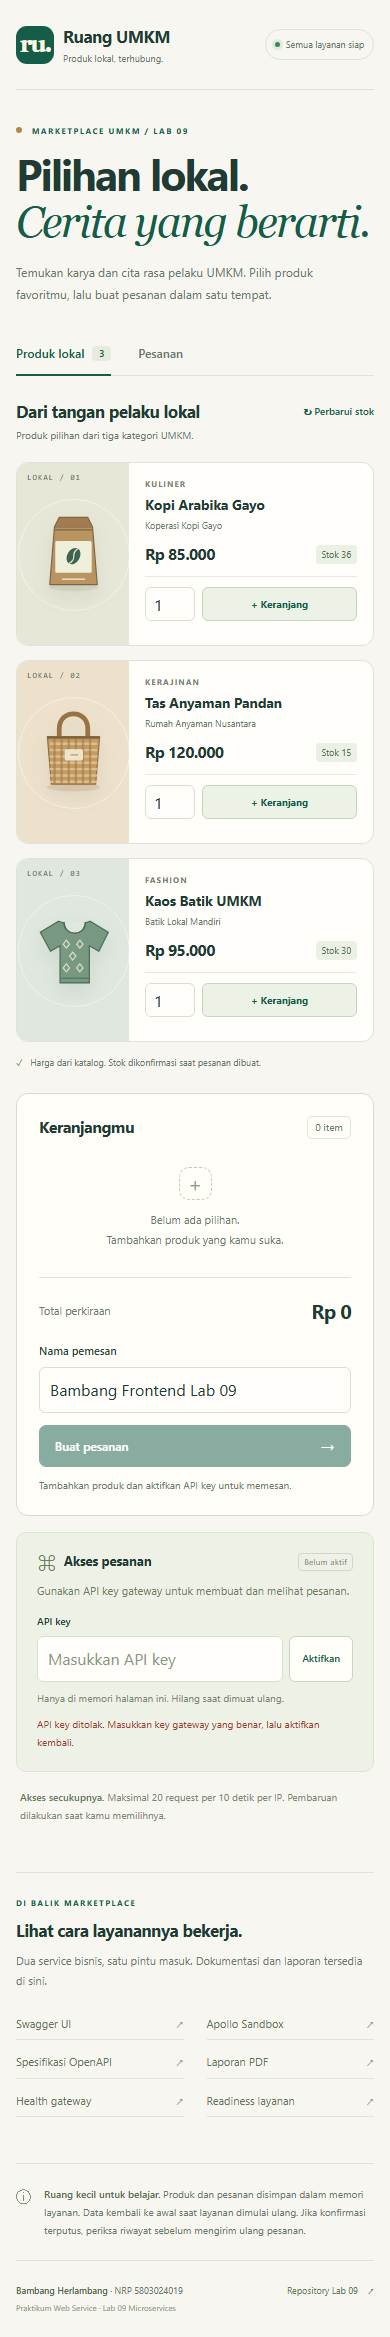
\includegraphics[width=.78\linewidth,height=.70\textheight,keepaspectratio,trim=0 0 0 1250bp,clip]{frontend-mobile.png}
\end{minipage}
\caption{Dua potongan berurutan dari satu screenshot mobile lokal:
katalog pada bagian atas dan form beserta pesan key ditolak pada bagian
bawah. Isi gambar tidak diubah.}
\end{figure}

\clearpage
\subsection{Swagger UI dan spesifikasi OpenAPI}
Swagger UI tersedia pada \code{/docs/} dan memuat spesifikasi
\code{/openapi.json}. Dokumentasi meliputi endpoint katalog, pesanan,
reservasi, GraphQL, health, serta respons error. Fungsi \textit{Authorize}
memungkinkan key dikirim untuk operasi yang memerlukannya tanpa
menanamkan nilai key dalam spesifikasi.

\begin{figure}[H]
\centering
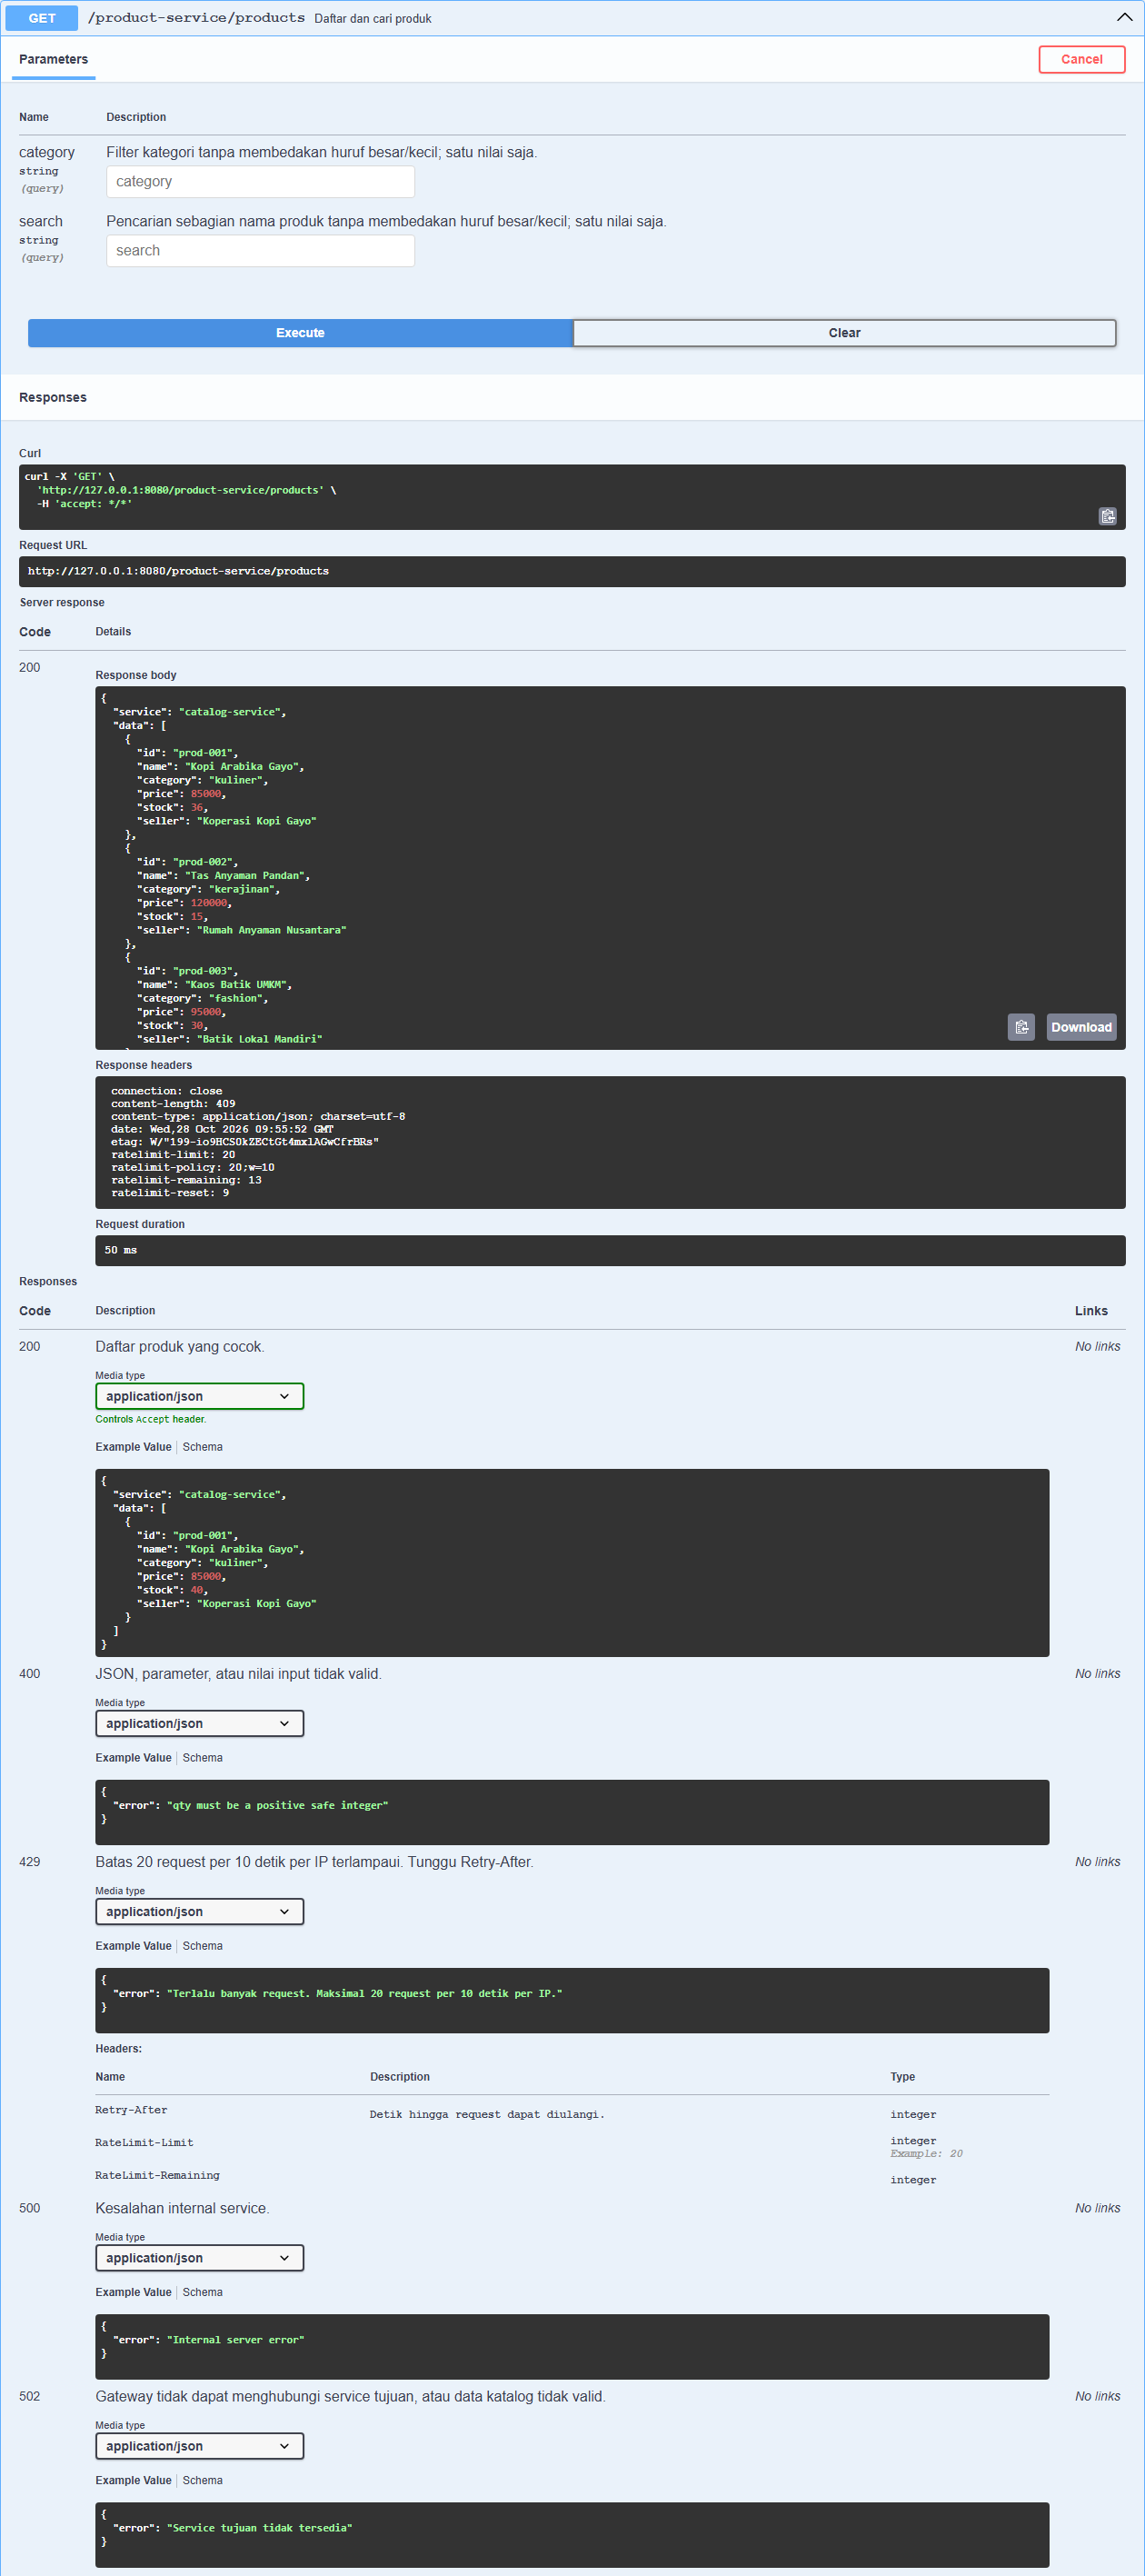
\includegraphics[width=\linewidth,height=.72\textheight,keepaspectratio,trim=0 1400bp 0 0,clip]{swagger-response.png}
\caption{Swagger Try it out pada gateway lokal mengembalikan HTTP 200
dan daftar produk. Area respons aktual ditampilkan; contoh respons statis
di bawahnya dipotong agar tidak tertukar sebagai bukti eksekusi.}
\end{figure}

Halaman dokumentasi tidak memakai kuota request API. Request yang dibuat
melalui Try it out tetap melewati route gateway, pemeriksaan key, dan
rate limit yang sama dengan klien lain.

\clearpage
\subsection{Apollo Sandbox dan GraphQL katalog}
Apollo Sandbox tersedia pada \code{/sandbox}. Endpoint GraphQL gateway:
\path{/product-service/graphql}. Halaman memakai Embedded Sandbox Apollo,
menyediakan query awal katalog, dan dapat membuka endpoint yang sama di
Apollo Studio. SDK tersebut memerlukan akses internet.

\begin{figure}[H]
\centering
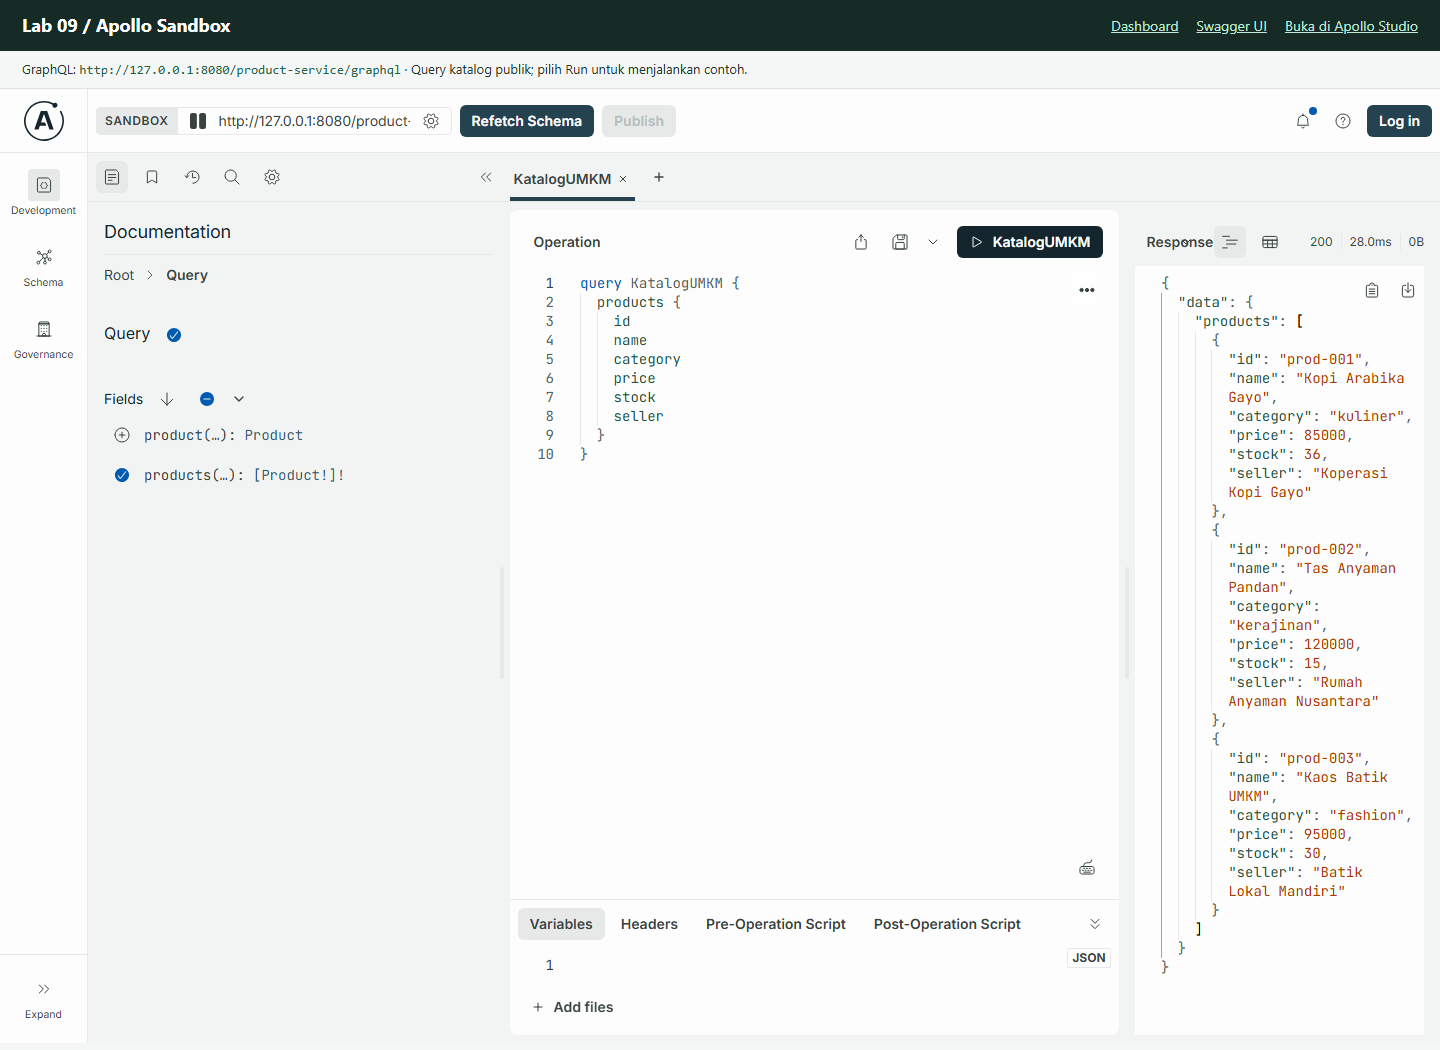
\includegraphics[width=\linewidth]{apollo-sandbox.png}
\caption{Operasi KatalogUMKM dijalankan melalui tombol Run pada Apollo
Sandbox lokal. Respons HTTP 200 menampilkan tiga produk beserta harga
dan stok; panel respons terlihat di sisi kanan.}
\end{figure}

\begin{lstlisting}
query KatalogUMKM {
  products { id name category price stock seller }
}
\end{lstlisting}
Hasil eksekusi tombol Run direkam dalam
\path{docs/evidence/ui/apollo-query.json}: status 200 dan tiga produk.
Query GraphQL katalog juga diverifikasi pada suite HTTP otomatis.
Berbagi akses lintas origin dibatasi pada endpoint GraphQL katalog yang
bersifat baca; kredensial pesanan tidak dibutuhkan untuk query tersebut.

\clearpage
\subsection{Konfigurasi deployment Render Free}
Deployment disiapkan pada \textbf{service Render terpisah khusus Lab 09},
menggunakan repository dan branch \code{main} Lab 09. Blueprint
\code{render.yaml} mendefinisikan satu instance Free yang menjalankan tiga
proses terpisah: gateway, katalog, dan pesanan. Hanya gateway yang
dipublikasikan; backend tetap pada loopback.

\begin{table}[H]
\small
\begin{tabularx}{\linewidth}{@{}L{3.7cm}Y@{}}
\toprule
Konfigurasi & Nilai \\
\midrule
Runtime / versi & Node.js 22 \\
Nama service & \code{prakwebservice-lab09-microservices} \\
Region / plan & Singapore / Free \\
Build & \code{npm ci --omit=dev} \\
Start & \code{npm start} \\
Health check & \code{/readyz} \\
Gateway & Host \code{0.0.0.0}, port dari platform, \code{TRUST_PROXY=1} \\
Backend & Host loopback; katalog port 3000, pesanan port 3001 \\
Key server & Digest SHA-256 melalui \code{API_KEY_SHA256} \\
\bottomrule
\end{tabularx}
\caption{Konfigurasi deployment pada blueprint Lab 09.}
\end{table}

\textbf{Status verifikasi publik.} Konfigurasi deployment Render Free
pada service terpisah telah disiapkan; verifikasi URL HTTPS, health,
frontend, Swagger, Apollo Sandbox, dan pesanan publik diperbarui setelah
layanan aktif. Bagian ini mencatat konfigurasi dan tidak menyatakan
deployment telah berhasil.

Collection Postman JSON dan environment lokal tersedia dalam
\path{docs/postman/}. Environment publik menggunakan base URL gateway
deployment, sementara nilai API key tetap diisi secara lokal oleh klien.
Data demo tetap bersifat in-memory pada deployment ini.


\clearpage
\section{Batasan konsistensi dan refleksi}
\subsection{Konsistensi data}
Validasi dan pengurangan stok dilakukan sinkron pada satu proses katalog,
tanpa jeda \code{await} di antara pemeriksaan dan mutasi. Produk berulang
digabungkan sehingga stok tidak terpotong berdasarkan pemeriksaan yang
terpisah. Batch yang ditolak tidak mengubah sebagian stok.

Jaminan tersebut terbatas pada operasi dalam katalog. Pengurangan stok
dan penyimpanan pesanan pada service lain belum menjadi transaksi
terdistribusi. Jika reservasi berhasil tetapi Order Service gagal
menyimpan pesanan, stok dapat berkurang tanpa pesanan yang terlihat oleh
klien. Timeout juga tidak membuktikan katalog belum memproses request.

Implementasi masih memakai memori; restart menghapus data proses terkait.
Idempotency key, masa berlaku reservasi, operasi kompensasi, database
persisten, dan koordinasi pembayaran merupakan pengembangan berikutnya.

\subsection{Refleksi}
Ketika Catalog Service mati, Order Service masih dapat menampilkan pesanan
karena riwayat pesanan dimiliki dan dibaca dari memorinya sendiri.
Hal ini memungkinkan pengguna memeriksa transaksi yang sudah tersimpan
sambil menunggu katalog pulih.
Jika stok telah dikurangi oleh reservasi tetapi pembuatan pesanan gagal
sesudahnya, stok dan pesanan dapat menjadi tidak konsisten sehingga perlu
mekanisme kompensasi atau reservasi dengan masa berlaku.
Dibanding monolit, microservices menambah panggilan jaringan, timeout,
kemungkinan kegagalan sebagian, serta pekerjaan konfigurasi dan pengujian.
Pemisahan tanggung jawab membantu membatasi dampak gangguan, tetapi
manfaat itu harus dibayar dengan pengelolaan konsistensi dan operasi
yang lebih rumit.

\subsection{Referensi dan berkas pengumpulan}
\begin{itemize}
\item Materi praktikum: \textit{Lab 09: Memecah Aplikasi Menjadi Microservices},
Web Service, Philipus Suryo Subandoro.
\item Repository implementasi: \repo.
\item Asal gateway: \href{https://github.com/academicbambang/prakwebservice-lab08-api-gateway}{repository Lab 08}.
\item Bukti mesin dan asal screenshot: \path{docs/evidence/lab09/}.
\item Collection Postman JSON: \path{docs/postman/}.
\item Sumber LaTeX mandiri dan gambar: \path{docs/latex-lab09/}.
\end{itemize}

\end{document}
